\lettrine{I}{n this chapter I present} the results of the models that have been specified in the previous chapters. I then explain how the results might be interpreted and what what it is we actually see in the results. But before coming to that, I look at some notable examples of the phenomenon in question to get a better understanding of the data at hand. This chapter will also include a discussion on the validity, reliability, and the robustness of the results, as there are many ways in which to model data, and even small changes may have rather large impacts on the results.

The main findings is that both my hypotheses were unsubstantiated; that linkages to China do not influence the level of freedom of expression in a country, and this holds regardless of regime type. I include several robustness checks to substantiate my conclusion.

\section{Examples}
\begin{table}[H]
\centering
\caption{Changes in freedom of expression and linkages to China}
\label{tab:change}
\begin{tabular}{lLp{15mm}lL}
\toprule
Country & \multicolumn{1}{c}{Freedom} & & Country & \multicolumn{1}{c}{Linkage} \\
\midrule
\cellcolor[HTML]{ff9214} Timor-Leste & 0.776 & & 
\cellcolor[HTML]{ff9214} Cambodia & 0.394 \\
Maldives & 0.636 & & Laos & 0.326 \\
Tunisia & 0.533 & & Turkmenistan & 0.314 \\
Libya & 0.531 & & Malaysia & 0.302 \\
Iraq & 0.510 & & Angola & 0.924 \\
\addlinespace
Hong Kong & -0.568 & & Tunisia & 0.018 \\
Venezuela & -0.670 & & Romania & -0.031 \\
Belarus & -0.735 & & Iran & -0.034 \\
Russia & -0.735 & & The Gambia & -0.067 \\
\cellcolor[HTML]{003F5C}\textcolor{white}{Nicaragua} & -0.869 &  &
\cellcolor[HTML]{003F5C}\textcolor{white}{North Korea} & -0.201 \\
\bottomrule
\multicolumn{5}{p{0.7\textwidth}}{\raggedright{\textit{For freedom score the the difference is measured between 1994 and 2024 \citep{coppedge_v-dem_2025}, while for linkage score it is the difference between 1994 and 2023 \citep{moyer_china-us_2021}.}}}
\end{tabular}
\end{table}

I want to start this section by examining some countries in greater detail to look at how our dependent and independent variables have changed over the time. Are there any signs that the main hypothesis is true? I have chosen four countries, based on their scores on the two main variables. These are: Timor-Leste, with the largest increase in freedom of expression score; Nicaragua, with the largest decrease in freedom of expression score; Cambodia, with the largest increase in linkages with China; and North Korea, with the largest decrease in linkages with China. The top and bottom five of both variables can be seen in Table \ref{tab:change}.

\begin{figure}[H]
    \centering
    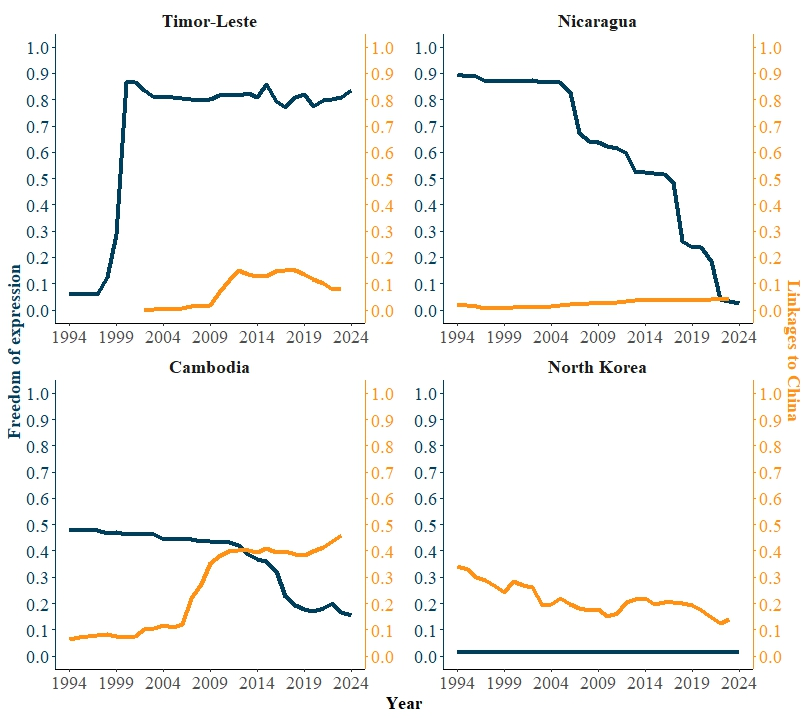
\includegraphics[width=\linewidth]{graphics/single_country_plots.jpeg}
    \caption{Change in linkages to China and freedom of expression}
    \label{fig:scp}
\end{figure}


\subsection{Timor-Leste}
Timor-Leste, also known as East Timor, is a small country in Southeast Asia, located on the east part of the island of Timor, which it shares with its larger neighbour Indonesia. The country has had a fraught history, that reached its climax in 1999, when the country became independent from Indonesia after 24 years of occupation \citep[p. 183]{kingsbury_democratic_2014} In Figure \ref{fig:scp} we can see that there is a large jump in the freedom of expression score in 1999, going from a score as low as 0.06 in 1997 to reaching a high of 0.87 in 2000. After which the score has decreased somewhat, but has generally been stable. While the FBIC index do not include scores before 2002, linkages to China only began rising around 2010, and with a mild increase, but this has not seemed to impact the freedom of expression to any great degree.

Timor-Leste shows that by far the most important factors are domestic, here related to independence. While this is not a boon for my theory, it also does not disconfirm it, as I do not expect linkages to China to be the only factor influencing freedom of expression. The linkage is also not very great, an I would not expect this to have a great impact in any case.

\subsection{Nicaragua}
Nicaragua is a rather poor Central American country, with a turbulent recent history. And recently, since 2006, the country has experienced a rapid democratic backsliding under the leadership of Daniel Ortega. The freedom of expression has seen a particularly steep decline, beating out both Russia and Belarus, however, these countries did have less of a way to fall.

While the linkages to China have slowly increased between 1994 and 2023, in absolute numbers they are quite low, and this again shows the importance of domestic factors when examining the decrease in freedom of expression.

\subsection{Cambodia}
Cambodia is a country on the Indochinese peninsula, which was not spared the ravages of the Cold War, hosting one of the most brutal regimes the world has ever seen in the communist Khmer Rouge. It did subsequently democratise; however, this was never very successful. Freedom of expression has taken a toll in this autocratising process, and in the period between 1994 and 2012, the country recorded a slow but persistent decline. This changed in 2012 as the score declined rapidly, before stabilising at a low level.

It is telling that the repression on freedom of expression began in earnest after a rapid increase in ties to China. The two lines in Figure \ref{fig:scp} seem almost to mirror each other, giving the superficial impression at least, that there is a connection. This is substantiated by the findings of \citet{loughlin_chinese_2021}.

\subsection{North Korea}
The last country I want to look at is North Korea, commonly labelled the hermit kingdom for its super-authoritarian and repressive regime. Its system is founded on self-reliance or Juche, with a strong cult of personality surrounding the ruling Kim clan. North Korea occupies the northern half of the Korean peninsula, and is almost entirely reliant on support from China. Even though Russia has become a closer partner after the 2022 invasion of Ukraine. 

\section{Hypothesis One} \label{sec:h1}
As a quick reminder, hypothesis one states that: \textit{thicker linkages to China will have a negative effect on the level of freedom of expression.} To study hypothesis one, I run a two-way fixed effects model with country and time fixed effects. I run several models, where I gradually include several control variables. The final model is equivalent to Equation \ref{equ:h1}. The gradual inclusion of controls serve to showcase the stability of the results. The results of this model is presented in Table \ref{tab:h1}. 

\subsection{Direct relationship between dependent and independent variables}
\begin{table}[H]
\centering
\resizebox{\textwidth}{!}{
\begin{talltblr}[         %% tabularray outer open
label=tab:h1,caption={Standard two-way fixed-effects models},
note{}={x p \num{< 0.1}, * p \num{< 0.05}, ** p \num{< 0.01}, *** p \num{< 0.001}},
]                     %% tabularray outer close
{                     %% tabularray inner open
colspec={Q[]Q[]Q[]Q[]Q[]Q[]Q[]},
column{2,3,4,5,6,7}={}{halign=c,},
column{1}={}{halign=l,},
hline{18}={1,2,3,4,5,6,7}{solid, black, 0.05em},
}                     %% tabularray inner close
\toprule
& \textbf{Model 1.1} & \textbf{Model 1.2} & \textbf{Model 1.3} & \textbf{Model 1.4} & \textbf{Model 1.5} & \textbf{Model 1.6} \\ \midrule %% TinyTableHeader
\SetCell{bg=Orange} Linkages to China &
\SetCell{bg=Orange} -0.081 & 
\SetCell{bg=Orange} -0.093 & 
\SetCell{bg=Orange} -0.069 & 
\SetCell{bg=Orange} -0.067 & 
\SetCell{bg=Orange} -0.111 & 
\SetCell{bg=Orange} -0.058 \\
& (0.132) & (0.134) & (0.127) & (0.128) & (0.130) & (0.111) \\
log(GDP per capita) &  & 0.009 & 0.001 & 0.008 & 0.016 & -0.003 \\
&  & (0.019) & (0.020) & (0.022) & (0.023) & (0.020) \\
Resource rents &  &  & 0.000 & 0.000 & 0.000 & 0.000 \\
&  &  & (0.001) & (0.001) & (0.001) & (0.001) \\
Aid &  &  &  & 0.001 & 0.001 & 0.002** \\
&  &  &  & (0.001) & (0.001) & (0.001) \\
Linkages (West) &  &  &  &  & -0.023* & -0.016x \\
&  &  &  &  & (0.012) & (0.009) \\
Electoral autocracy &  &  &  &  &  & 0.085** \\
&  &  &  &  &  & (0.030) \\
Electoral democracy &  &  &  &  &  & 0.238*** \\
&  &  &  &  &  & (0.034) \\
Liberal democracy &  &  &  &  &  & 0.285*** \\
&  &  &  &  &  & (0.037) \\
Num.Obs. & 5154 & 5150 & 4657 & 4648 & 4648 & 4648 \\
Std.Errors & by: country & by: country & by: country & by: country & by: country & by: country \\
R2 Adj. & 0.874 & 0.874 & 0.882 & 0.883 & 0.883 & 0.907 \\
R2 Within Adj. & 0.001 & 0.001 & 0.000 & 0.003 & 0.008 & 0.208 \\
FE: country & X & X & X & X & X & X \\
FE: year & X & X & X & X & X & X \\
\bottomrule
\end{talltblr}
}
\end{table} 

Model one in Table \ref{tab:h1} shows the effect of linkages to China on freedom of expression, with the freedom of expression scores being lagged by one year to exclude reversed causation. In Table \ref{tab:h1_lag} I run Model 6 from Table \ref{tab:h1} with different lags, to gauge the impact of lags. 

It can be clearly surmised from Table \ref{tab:h1} that linkages to China does not have a direct impact on freedom of expression scores in the aggregate. While the sign of the linkage variable is indeed negative, the standard error is quite large, in most cases being twice the size of the estimated effect. There are a few more things to note, first, that the coefficient for GDP per capita is non-significant, second, that only aid and regime type is significant, and this only in Model 6, and third, that the coefficient for the variable measuring linkages to the West is negative, but this is also not significant. I will discuss these findings in the next chapter, however, they should be noted here.

In Model 1.1, I simply regress the independent variable on the dependent. This yields a negative coefficient, but too large a standard error for making anything of this estimate. While the main dataset includes 5,154 complete observations over the dependent and independent variables, I lose 169 observations when lagging the dependent variable one year. In Model 1.2, I add a logarithmically transformed GDP per capita variable to the model, observing that this does not make the results significant. I additionally lose 4 observations. I then proceed to Model 1.3 where I add in rents from natural resources, measured as a percentage of GDP. Here again we see no significant changes to the estimates; however, we lose 480 more observations. In Model 1.4 I add a variable measuring the aid a country receives as a percent of GNI. This also has no significant impact on the coefficients, and I lose an additional 20 observations, bringing the number of observations to 4,481. Model 1.5 includes a variable measuring linkages to Western countries. The coefficient is not significant, but it is interesting that my data shows a negative correlation between linkages to the west and freedom of expression. To the last model, Model 1.6, I add a factor variables dividing the observations into regime type. As regime type is a variable constructed partly from the dependent variable, and the reference category is autocracies, it is unsurprising that these factor variables are strongly positive and significant.

\subsection{Relationship between dependent variable and change in the independent variable}

\begin{table}[H]
\centering
\resizebox{\textwidth}{!}{
\begin{talltblr}[         %% tabularray outer open
label=tab:h1_delta,caption={Models using change in the independent variable},
note{}={x p \num{< 0.1}, * p \num{< 0.05}, ** p \num{< 0.01}, *** p \num{< 0.001}},
]                     %% tabularray outer close
{                     %% tabularray inner open
colspec={Q[]Q[]Q[]Q[]Q[]Q[]Q[]},
column{2,3,4,5,6,7}={}{halign=c,},
column{1}={}{halign=l,},
hline{18}={1,2,3,4,5,6,7}{solid, black, 0.05em},
}                     %% tabularray inner close
\toprule
& Model 1.7 & Model 1.8 & Model 1.9 & Model 1.10 & Model 1.11 & Model 1.12 \\ \midrule %% TinyTableHeader
\SetCell{bg=Orange} Linkages to China & 
\SetCell{bg=Orange} 0.185x & 
\SetCell{bg=Orange} 0.186x & 
\SetCell{bg=Orange} 0.176x & 
\SetCell{bg=Orange} 0.193x & 
\SetCell{bg=Orange} 0.191x & 
\SetCell{bg=Orange} 0.136 \\
& (0.101) & (0.101) & (0.105) & (0.108) & (0.107) & (0.088) \\
log(GDP per capita) &  & 0.006 & -0.001 & 0.006 & 0.012 & -0.005 \\
&  & (0.019) & (0.020) & (0.022) & (0.023) & (0.020) \\
Resource rents &  &  & 0.000 & 0.000 & 0.000 & 0.000 \\
&  &  & (0.001) & (0.001) & (0.001) & (0.001) \\
Aid &  &  &  & 0.001 & 0.001x & 0.002** \\
&  &  &  & (0.001) & (0.001) & (0.001) \\
Linkages (West) &  &  &  &  & -0.020x & -0.015x \\
&  &  &  &  & (0.011) & (0.009) \\
Electoral autocracy &  &  &  &  &  & 0.083** \\
&  &  &  &  &  & (0.030) \\
Electoral democracy &  &  &  &  &  & 0.234*** \\
&  &  &  &  &  & (0.034) \\
Liberal democracy &  &  &  &  &  & 0.277*** \\
&  &  &  &  &  & (0.036) \\
Num.Obs. & 4968 & 4964 & 4478 & 4471 & 4471 & 4471 \\
Std.Errors & by: country & by: country & by: country & by: country & by: country & by: country \\
R2 Adj. & 0.877 & 0.877 & 0.884 & 0.885 & 0.886 & 0.908 \\
R2 Within Adj. & 0.004 & 0.004 & 0.004 & 0.007 & 0.011 & 0.206 \\
FE: country & X & X & X & X & X & X \\
FE: year & X & X & X & X & X & X \\
$\Delta$ Years Linkages & 3 & 3 & 3 & 3 & 3 & 3 \\
\bottomrule
\end{talltblr}
}
\end{table} 

While in Table \ref{tab:h1} I directly regressed the independent variable on the dependent, in Table \ref{tab:h1_delta} I regress the three year change in the independent variable on the dependent variable. I do this because I am interested in looking at the how a change in linkages might affect freedom of expression, not just whether high values on the linkage-variable go together with low values on the freedom of expression-variable. The other specifications are the same, using two-way fixed-effects and a one year lag on the dependent variable. This model is equivalent to Equation \ref{equ:h2}.

The first model, Model 1.7, regresses change in linkages to China on the freedom of expression score lagged by one year. This has a total of 4,800 observations. This configuration, in contrast to directly regressing the linkage and freedom scores on each other, shows a positive relationship between linkages to China and freedom of expression. That is to say that an increase in linkages to China is associated with less repression of freedom of expression. However, this is only significant on the ten per cent level, indicating that this should be interpreted with a great deal of scepticism. Model 1.8 adds the logarithmically transformed GDP per capita variable, the significance is equivalent to Model 1.7, and we lose four observations. In Model 1.9 I add resource rents to the model, with the effect that it is not longer significant on the ten per cent level, and we lose 473 observations. To Model 1.10 is added the aid variable, which returns the coefficient back to significant on the ten per cent level, and in the process an additional 22 observations are lost, giving the rest of the models to a baseline of 4,305 observations. To Model 1.11 I add the variable controlling for linkages to the West. The coefficient of linkages to China remains positive and significant on the ten per cent level, while the variable controlling for linkages to the West is again negative, but not significant. The last model in Table \ref{tab:h1_delta} is Model 1.12, which contains the factorised regime variable. The coefficient of linkages to China is no longer significant, while the regime variables are, for the same reasons as above, positive and significant.

The main takeaways of Table \ref{tab:h1_delta} is that the results are unstable and not significant. While the results are significant on the ten percent level, this is lower than the commonly accepted threshold of five per cent, and means that one in ten times our model would reject the null-hypothesis even when it was right. This is quite often, and we should not read anything significant into the results, even if we should note the limited plausibility of this result and the implications it has on our theory, which states the opposite of what here is presented.

\section{Hypothesis two and three} \label{sec:h2}
In hypothesis two and three, I set out to study if the linkage effect is regime dependent. It will be remembered from the last chapter of the theory section that I hypothesise that consolidated regimes would be unlikely to be affected by linkages to China, while hybrid regimes are likely to be affected. In this section I add an interaction term between the linkages to China variable and the regime variable. The resulting interactions shows the effect of linkages on a certain type of regime, with consolidated autocracies being the reference category.

\subsection{Standard relationship with an interaction}

\begin{table}[H]
\centering
\resizebox{\textwidth}{!}{
\begin{talltblr}[         %% tabularray outer open
label=tab:h2,caption={Models with interaction between linkages and regime types},
note{}={x p \num{< 0.1}, * p \num{< 0.05}, ** p \num{< 0.01}, *** p \num{< 0.001}},
]                     %% tabularray outer close
{                     %% tabularray inner open
colspec={Q[]Q[]Q[]Q[]Q[]Q[]},
column{2,3,4,5,6}={}{halign=c,},
column{1}={}{halign=l,},
hline{24}={1,2,3,4,5,6}{solid, black, 0.05em},
}                     %% tabularray inner close
\toprule
& Model 2.1 & Model 2.2 & Model 2.3 & Model 2.4 & Model 2.5 \\ \midrule %% TinyTableHeader
\SetCell{bg=Orange} Linkages to China & 
\SetCell{bg=Orange} -0.047 & 
\SetCell{bg=Orange} -0.025 & 
\SetCell{bg=Orange} -0.096 & 
\SetCell{bg=Orange} -0.096 & 
\SetCell{bg=Orange} -0.124 \\
& (0.218) & (0.230) & (0.256) & (0.249) & (0.252) \\
Electoral autocracy & 0.094** & 0.097** & 0.071* & 0.075* & 0.074* \\
& (0.036) & (0.036) & (0.034) & (0.034) & (0.034) \\
Electoral democracy & 0.261*** & 0.265*** & 0.234*** & 0.237*** & 0.235*** \\
& (0.039) & (0.040) & (0.039) & (0.039) & (0.039) \\
Liberal democracy & 0.313*** & 0.318*** & 0.292*** & 0.295*** & 0.288*** \\
& (0.041) & (0.042) & (0.043) & (0.043) & (0.041) \\
\SetCell{bg=Orange} China x El.Aut. & 
\SetCell{bg=Orange} -0.044 & 
\SetCell{bg=Orange} -0.045 & 
\SetCell{bg=Orange} 0.113 & 
\SetCell{bg=Orange} 0.117 & 
\SetCell{bg=Orange} 0.115 \\
& (0.290) & (0.294) & (0.312) & (0.301) & (0.299) \\
\SetCell{bg=Orange} China x El.Dem. & 
\SetCell{bg=Orange} -0.090 & 
\SetCell{bg=Orange} -0.092 & 
\SetCell{bg=Orange} -0.018 & 
\SetCell{bg=Orange} -0.012 & 
\SetCell{bg=Orange} -0.004 \\
& (0.253) & (0.256) & (0.274) & (0.266) & (0.266) \\
\SetCell{bg=Orange} China x Lib.Dem. & 
\SetCell{bg=Orange} -0.238 & 
\SetCell{bg=Orange} -0.268 & 
\SetCell{bg=Orange} -0.207 & 
\SetCell{bg=Orange} -0.207 & 
\SetCell{bg=Orange} -0.126 \\
& (0.260) & (0.277) & (0.291) & (0.280) & (0.280) \\
log(GDP per capita) &  & -0.013 & -0.019 & -0.011 & -0.005 \\
&  & (0.017) & (0.018) & (0.019) & (0.020) \\
Resource rents &  &  & 0.000 & 0.000 & 0.000 \\
&  &  & (0.001) & (0.001) & (0.001) \\
Aid &  &  &  & 0.002** & 0.002** \\
&  &  &  & (0.001) & (0.001) \\
Linkages (West) &  &  &  &  & -0.014 \\
&  &  &  &  & (0.009) \\
Num.Obs. & 5154 & 5150 & 4657 & 4648 & 4648 \\
Std.Errors & by: country & by: country & by: country & by: country & by: country \\
R2 Adj. & 0.902 & 0.901 & 0.905 & 0.907 & 0.907 \\
R2 Within Adj. & 0.216 & 0.217 & 0.201 & 0.207 & 0.209 \\
FE: country & X & X & X & X & X \\
FE: year & X & X & X & X & X \\
\bottomrule
\end{talltblr}
}
\end{table} 

Table \ref{tab:h2} is the same as table Table \ref{tab:h1}, but this time using an interaction term between the linkages to China variable and regime type. This have the unfortunate effect of complicating the model, however, we can now see the effect that linkages have on each regime type. To simplify the reading of the table, we are going to focus most of our attention on the highlighted rows, as these are the main coefficients we are interested in.

There are some interesting differences from the models being run in Section \ref{sec:h1}, but the results are not statistically significant. While it is consistently estimated that linkages to China have a negative effect on freedom of expression for consolidated regimes, the coefficients for hybrid regimes are less stable, becoming positive for electoral autocracies in Model 2.3 and positive for electoral democracies in Model 2.4.

\subsection{Relationship with change in the independent variable and an interaction}

\begin{table}[!hbt]
\centering
\resizebox{\textwidth}{!}{
\begin{talltblr}[         %% tabularray outer open
label=tab:h2_delta,caption={Models with interaction between change in linkages and regime type},
note{}={x p \num{< 0.1}, * p \num{< 0.05}, ** p \num{< 0.01}, *** p \num{< 0.001}},
]                     %% tabularray outer close
{                     %% tabularray inner open
colspec={Q[]Q[]Q[]Q[]Q[]Q[]},
column{2,3,4,5,6}={}{halign=c,},
column{1}={}{halign=l,},
hline{24}={1,2,3,4,5,6}{solid, black, 0.05em},
}                     %% tabularray inner close
\toprule
& Model 2.6 & Model 2.7 & Model 2.8 & Model 2.9 & Model 2.10 \\ \midrule %% TinyTableHeader
\SetCell{bg=Blue} \textcolor{white}{Linkages to China} & 
\SetCell{bg=Blue} \textcolor{white}{0.217x} & 
\SetCell{bg=Blue} \textcolor{white}{0.219x} & 
\SetCell{bg=Blue} \textcolor{white}{0.242*} & 
\SetCell{bg=Blue} \textcolor{white}{0.305*} & 
\SetCell{bg=Blue} \textcolor{white}{0.300*} \\
& (0.111) & (0.111) & (0.120) & (0.134) & (0.134) \\
Electoral autocracy & 0.083** & 0.087** & 0.077* & 0.081** & 0.080** \\
& (0.030) & (0.030) & (0.030) & (0.030) & (0.030) \\
Electoral democracy & 0.246*** & 0.250*** & 0.229*** & 0.233*** & 0.231*** \\
& (0.033) & (0.033) & (0.033) & (0.034) & (0.034) \\
Liberal democracy & 0.289*** & 0.293*** & 0.277*** & 0.281*** & 0.278*** \\
& (0.035) & (0.035) & (0.037) & (0.037) & (0.036) \\
\SetCell{bg=Orange} China x El.Aut. & 
\SetCell{bg=Orange} -0.056 & 
\SetCell{bg=Orange} -0.057 & 
\SetCell{bg=Orange} -0.095 & 
\SetCell{bg=Orange} -0.146 & 
\SetCell{bg=Orange} -0.147 \\
& (0.179) & (0.179) & (0.184) & (0.191) & (0.190) \\
\SetCell{bg=Blue} \textcolor{white}{China x El.Dem.} & 
\SetCell{bg=Blue} \textcolor{white}{-0.294*} & 
\SetCell{bg=Blue} \textcolor{white}{-0.292*} & 
\SetCell{bg=Blue} \textcolor{white}{-0.303*} & 
\SetCell{bg=Blue} \textcolor{white}{-0.380*} & 
\SetCell{bg=Blue} \textcolor{white}{-0.369*} \\
& (0.135) & (0.136) & (0.137) & (0.148) & (0.149) \\
\SetCell{bg=Blue} \textcolor{white}{China x Lib.Dem.} & 
\SetCell{bg=Blue} \textcolor{white}{-0.370**} & 
\SetCell{bg=Blue} \textcolor{white}{-0.373**} & 
\SetCell{bg=Blue} \textcolor{white}{-0.364**} & 
\SetCell{bg=Blue} \textcolor{white}{-0.456**} & 
\SetCell{bg=Blue} \textcolor{white}{-0.406**} \\
& (0.134) & (0.134) & (0.134) & (0.144) & (0.146) \\
log(GDP per capita) &  & -0.013 & -0.018 & -0.009 & -0.005 \\
&  & (0.017) & (0.018) & (0.019) & (0.020) \\
Resource rents &  &  & 0.000 & 0.000 & 0.000 \\
&  &  & (0.001) & (0.001) & (0.001) \\
Aid &  &  &  & 0.002** & 0.002** \\
&  &  &  & (0.001) & (0.001) \\
Linkages (West) &  &  &  &  & -0.012 \\
&  &  &  &  & (0.009) \\
Num.Obs. & 4968 & 4964 & 4478 & 4471 & 4471 \\
Std.Errors & by: country & by: country & by: country & by: country & by: country \\
R2 Adj. & 0.903 & 0.903 & 0.907 & 0.909 & 0.909 \\
R2 Within Adj. & 0.215 & 0.217 & 0.199 & 0.209 & 0.210 \\
FE: country & X & X & X & X & X \\
FE: year & X & X & X & X & X \\
$\Delta$ Years Linkages & 3 & 3 & 3 & 3 & 3 \\
\bottomrule
\end{talltblr}
}
\end{table} 

Table \ref{tab:h2_delta} repeats Table \ref{tab:h1_delta}, but as in the above section, I include an interaction term between linkages to China and regime type. This is by far the most interesting result so far, as we have significant results on the five per cent level. Before proceeding with the analysis, I will make a quick rejoinder on statistical significance, because this result should not be overstated. Significance is an arbitrarily chosen threshold where we consider a result to be plausible enough that we accept it as `true.' The most accepted threshold goes at the five per cent level, meaning that if we do the study 100 times, we can expect that in 95 of them of them we end up with a coefficient that is different from zero, and we can plausibly reject the null-hypothesis. But even if in this case there can be a lot of uncertainty in the result, so any inferences should be done with this in mind. The results in Table \ref{tab:h2_delta} have quite large standard errors, so we should be careful when analysing the results.

The coefficients of linkages to China, which indicates the effect of linkages to China for a consolidated autocracy, is positive and not significant across the five models, with the effect size increasing for each added control variable. The same is the case for electoral autocracies, however, her the effect size decreases when adding controls. For democracies the sign is reversed, but the models are still not significant for electoral democracies. There is also a trend where both liberal and electoral democracies have their effect sizes reduced when adding in controls for GDP per capita and resource rents (Models 2.7 and 2.8), however, they do a sudden jump when adding in a control variable for aid (Model 2.9), before decreasing again when adding in control for linkages to the West (Model 2.10). (DISCUSS!!)

The most interesting results are the coefficients showing the effect of linkages to China on liberal democracies. In Models 2.6, 2.7, and 2.8, the coefficients are negative and only significant on the ten per cent level. These are so far the strongest indications there are for linkages to China having a negative impact on other countries. These effects are then strengthened in Models 2.9 and 2.10, where the effect crosses the commonly held threshold of statistical significance. The standard errors are still fairly substantial, however, they are a little under half the size of the estimated effect, but for Model 2.10 this is only by the breadth of a hair. Indicating that we should be careful not to make too strong claims. The size of the effect, on the other hand, is substantial. The standard deviation of freedom of expression, as will be remembered from Table \ref{tab:summary}, is 0.29, making a one unit increase in linkages to China almost equivalent to a drop equivalent to a standard deviation in the freedom of expression score. (INCLUDE AN EXAMPLE, and how much is a units increase in FBIC-score? If it is 0 to 1, it might not be that much:/)

\section{Robustness Tests} \label{sec:robust}
To test the robustness of the results, I run several different model specifications to see how well the models hold up to scrutiny. While I present the results here, all the tables referred to in this section can be found in Appendix \ref{apn:robust}. In all I make four changes to my models, to assess how all the models in Tables \ref{tab:h1}, \ref{tab:h1_delta}, \ref{tab:h2}, and \ref{tab:h2_delta} stand up to different forms of scrutiny. First I look at the impact of different time lags on all the models in the four tables presented above. Second I investigate how removing the one year time lag impacts the models. Third I make two tables using models 1.6 and 2.6 to look at how the length of time used for the change in linkages variable impacts the estimation. Finally I replace the FBIC-variable with the bandwidth variable also featured in the FBIC dataset \citep{moyer_china-us_2021}. Doing this ensures that the variable are consistent in their results. I find that they are generally consistent, but with some differences. Notable among them are Tables \ref{tab:h2_delta_x_lag} and \ref{tab:h2_bandwidth_delta} which gave significant results.

\subsection{Models with different lags}
I include four additional tables showing different amounts of time lag in Appendix \ref{apn:models}. These are Tables \ref{tab:h1_lag}, \ref{tab:h1_delta_lag}, \ref{tab:h2_lag}, and \ref{tab:h2_delta_lag}. The reason for including these can be seen in Figure \ref{fig:scp}, where Cambodia shows a conspicuous amount of lag between an increase in linkages and its effect on freedom of expression. To limit the number of models, I specifically use Models 1.6, 1.12, 2.5, and 2.10, with lags from one to five years. The third model is the model used in the tables included above. 

I find that the addition of greater time lags does not make the results significant. On the contrary, what I find is that the greater the lag, the more uncertain the estimates of the coefficients become. Thus, the only case it was positive, was in the model using a lag of one year. This is Model 2.10 in Table \ref{tab:h2_delta} or Model A.1.16 in Table \ref{tab:h2_delta_lag}. The trend to diminishing significance  is in hindsight obvious, as any effect will diminish with time. However, in light of the case of Cambodia in the section above, it makes sense to enquire into the effect of time-lags, as effects may take time to manifest themselves.

\subsection{Models without lag on the dependent variable}
I next include four more tables running the four main tables of this chapter without lag. I do this to check if the effect might be immediate. I do not expect it to be, however, large discrepancies when doing this should be investigated further. As a caveat to this, it is somewhat likely that the models using change in the linkages---instead of the absolute size of them---can impact the estimates of the coefficients. As I have already noted, the effect is stronger the smaller the lag, and, in the case of change in the independent variable, the possibility of reversed causation is excluded. This means that we should take very seriously any change in the estimates when using change in linkages as the main independent variable.

Tables \ref{tab:h1_x_lag}, \ref{tab:h1_delta_x_lag}, and \ref{tab:h2_x_lag} shows no significant changes from the models in the analysis chapter. The estimated coefficients are a little different, but no major changes. Table \ref{tab:h2_delta_x_lag}, however, shows a stronger relationship than does Table \ref{tab:h2_delta} above. As indicated above, the removal of the time lag has made the coefficients for some of the variables we are interested in stronger. The interaction term between linkages to China and liberal democracies are now negative and statistically significant across all the models. In addition, the coefficients for the interaction term between linkages to China and electoral democracies becomes statistically significant in models A.2.21 and A.2.22, showing that more linkages to China leads to a decrease in freedom of expression score. Interestingly, Models A.2.21 and A.2.22 also shows the interaction term between linkages to China and consolidated autocracies to be significant, but this relationship is positive, indicating that an increase in linkages to China is likely to have a positive effect on freedom of expression for the most autocratic states.

\subsection{Models with different number of years of change}
The third specification I run, takes its basis in the change in linkages to China. I run five models with different number of years of change for Models 1.12 and 2.10. the models have changes from one to five years.

I find that for the models without interaction there is almost no significant changes, and there is thus not much to say about Table \ref{tab:h1_diff_delta}. Table \ref{tab:h2_diff_delta} is a bit more interesting. Here we see that the the interaction between linkages and liberal democracy is only significant when using three or more years of change. This makes sense, as there is much more variation in the changes when the time-span is shorter. At three years of change the estimated coefficients are significant. After this point the  coefficients increase in size, but so do the standard errors, i.e., the uncertainty of our estimates.

\subsection{Bandwidth}
The last specification I run uses the `bandwidth' variable which is one of the two parts that make up the FBIC index main variable. I include models using this variable to see how removing the importance of the linkages affects the estimations. Bandwidth measures the number of linkages, but not how important these are to the partner of China. According to \citet{levitsky_linkage_2006}, linkages are the main way through which democracy can be spread, with leverage mainly working to strengthen the effects of the linkages. The number of linkages than, is more important than their size according to this theory. On this basis I include models using bandwidth to check the stability of the results. Again, I rerun all the models in the four main tables of this section.

What I find when using bandwidth as the independent variable, is that the models from Table \ref{tab:h1} barely changes (see Table \ref{tab:h1_bandwidth}). The same is true for Table \ref{tab:h2} (see Table \ref{tab:h2_bandwidth}) However, there are differences when using change in the bandwidth variable. In Table \ref{tab:h1_bandwidth_delta}, the linkages to China variable becomes statistically significant and positive. This is to say that an increase in the number of linkages to China is associated with an increase in the freedom of expression score. On the other hand, in Table \ref{tab:h2_bandwidth_delta}, I find that using change in bandwidth with the regime interaction term removes the statistical significance that we saw in Table \ref{tab:h2_delta}. This means that an increase in the number of linkages, is not associated with any significant change for any particular regime type. 

\textbf{Question for Ina and Felix: should I use the table without lag on the dependent variables when I use the linkage variable measuring change? (See Table \ref{tab:h1_delta_x_lag} and \ref{tab:h2_delta_x_lag})}

\section{Summary}
To summarise this chapter, I have run several models looking at the relationship between linkages to China and freedom of expression. Generally, there is not much evidence that linkages to China have any great impact on freedom of expression in other countries. There was one significant result: an increase in linkages to China has a negative effect on freedom of expression in liberal democracies. This goes against hypothesis two, which states that consolidated regimes are less likely to be influenced by linkages. At the same time it gives conditional support to hypothesis one; that thicker linkages to China has a negative effect on freedom of expression. However, the models are not stable, and Table \ref{tab:h1_bandwidth_delta} even saw linkages to China having a positive impact on freedom of expression. In the next chapter I will discuss what these findings means for my own study and for the study of autocratisation more generally.